\subsection{Solar irradiation on the Earth's surface} \label{sec:solar_irradiation_on_earths_surface}
Compared to equation (\ref{eq:e_sun}), determining the Sun's irradiance arriving on the surface of Earth is rather complex.\footnote{The authors of the article \cite{Babikir:2020} use the Capderou method to model the incident solar radiation on Earth. In the articles\cite{Appelbaum:1990, Appelbaum:1992} this topic is investigated with a different method for the planet Mars.} Precise calculations depend on many different factors such as the changing angular relationship between the Sun and Earth throughout the year, the composition of Earth's atmosphere -- which changes the Sun's spectrum due to absorbtion and scattering effects -- and many more \cite{Landis:1995, Mertens:2015, Wagner:2018}. 

With solar resource maps however, this problem can be circumvented. They are based on satellite and atmospheric solar irradiance models and meteorological data that were designed and collected over several years. By using these maps the compromise is made that the following calculations and estimates are performed with average irradiance values instead of exact ones. Figures \ref{fig:ghi_austria} and \ref{fig:dni_austria} provided by \cite{SolargisMaps:2020, GlobalSolarAtlas:2020} show the solar resource maps of the long term average global horizontal and direct normal irradiation, from 1994 until 2018, of Austria. The scale below the maps shows daily and annual total irradiation in $\left( \mathrm{kWh}\mathrm{m}^{-2} \right)$ \cite{MeteorologicalModeling:2020, SolarRadiationModeling:2020, SolargisData:2020}. 
\begin{figure}[h!]
	\centering
  	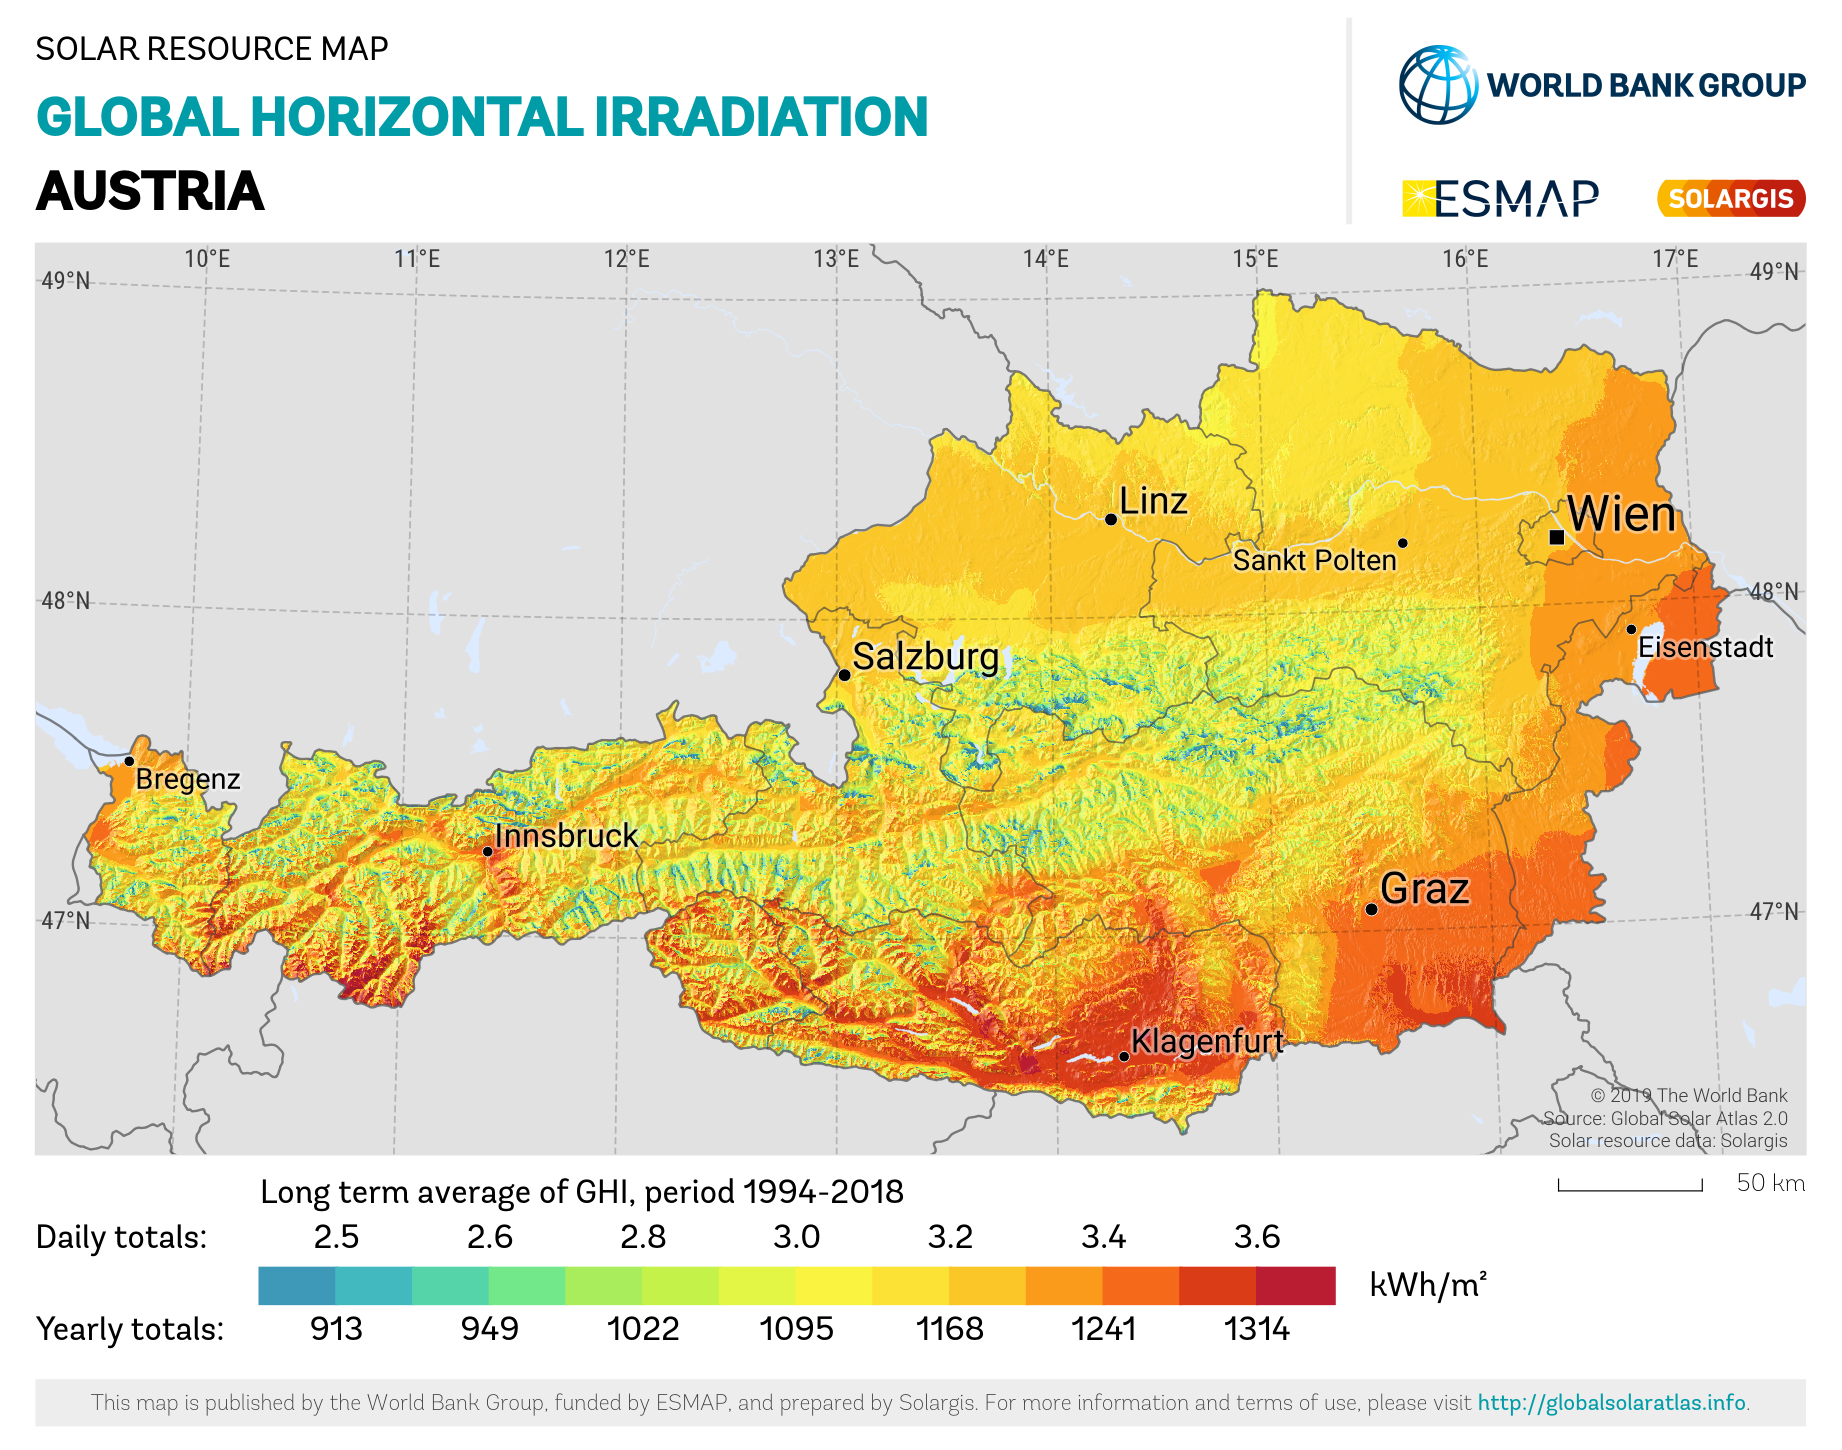
\includegraphics[width = 0.96\textwidth]{solar_maps/austria/austria_ghi}
  	\caption{Solar resource map of the long term average global horizontal irradiation of Austria. (Image credit: \cite{GlobalSolarAtlas:2020, Solargis:2021})}
	\label{fig:ghi_austria}
\end{figure}
\begin{figure}[h!]
	\centering
  	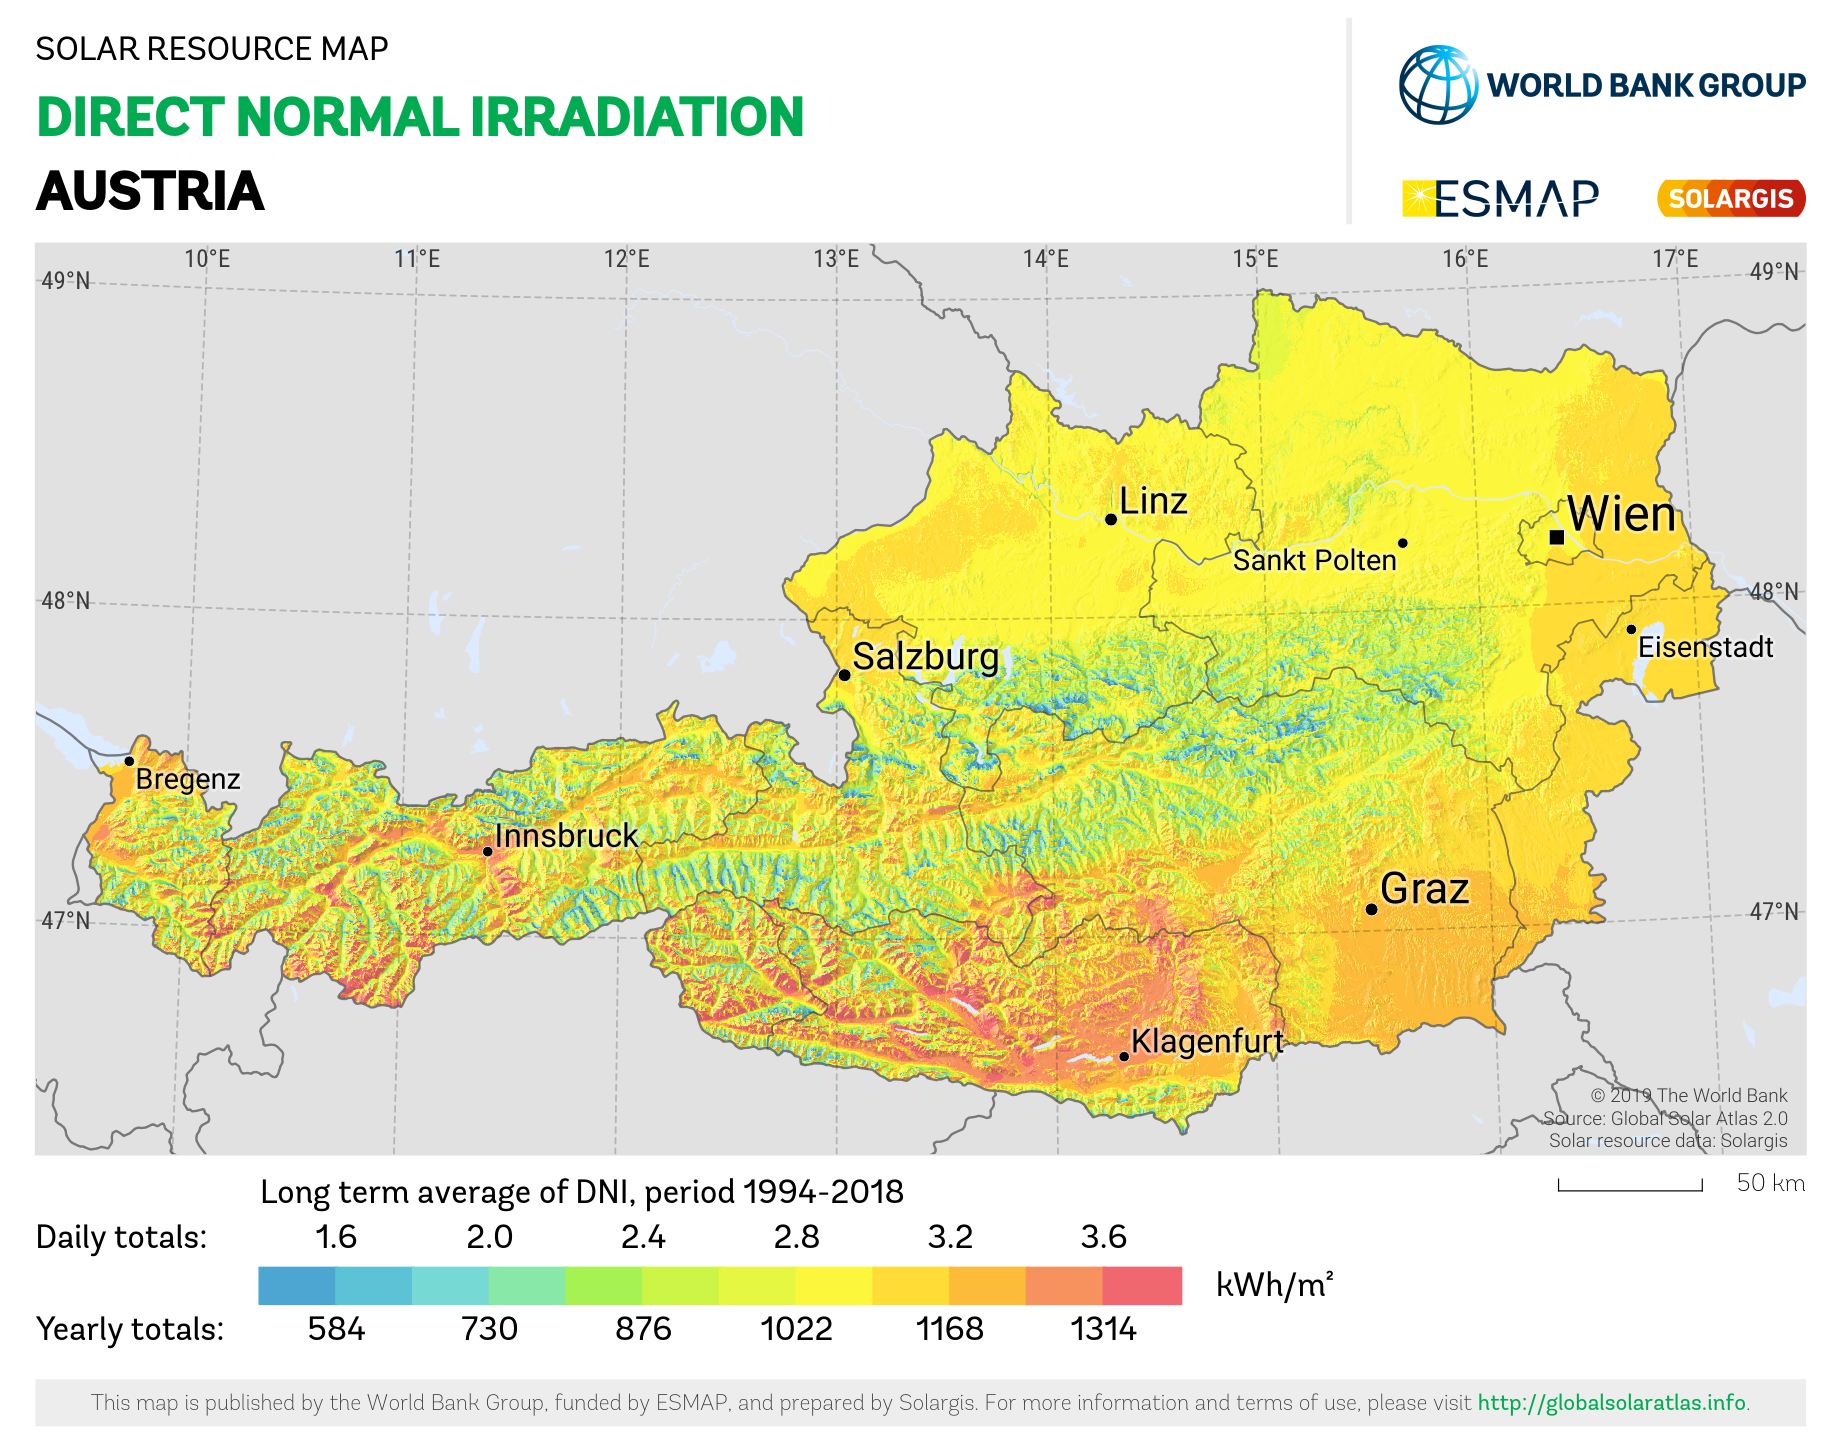
\includegraphics[width = 0.96\textwidth]{solar_maps/austria/austria_dni}
	\caption{Solar resource map of the long term average direct normal irradiation of Austria. (Image credit: \cite{GlobalSolarAtlas:2020, Solargis:2021})}
	\label{fig:dni_austria}
\end{figure}

It can be clearly seen that the values for both the global horizontal and the direct normal irradiation tend to be higher in the south and lower in the north of Austria. This can be partly explained by a greater latitude $\varphi$ which results in a lower altitude of the Sun $\gamma_{\mathrm{S}}$ during the winter months on the northern hemisphere ($\delta < 0$). Because of this, the Sun's incoming rays need to penetrate a thicker atmopshere and it is visible above the horizon for a shorter period of time over the course of the day. For locations in the south, such as the region around Klagenfurt, daily global horizontal irradiation totals of up to $3,50\mathrm{kWh}\mathrm{m}^{-2}$ and direct normal irradiation totals of up to $3,55\mathrm{kWh}\mathrm{m}^{-2}$ and higher can be expected, whereas loactions in the north, such as the region around Linz, only reach daily global horizontal irradiation totals of around $3,25\mathrm{kWh}\mathrm{m}^{-2}$ and daily direct normal irradiation totals of around $2,9\mathrm{kWh}\mathrm{m}^{-2}$. Another notable feature are valleys bordered by mountains in the south. In these valleys, and on the bounding north-facing mountain slopes, the daily global horizontal irradiation totals drop to less than $2,5\mathrm{kWh}\mathrm{m}^{-2}$ and the daily direct normal irradiation totals drop even further down to around $1,5\mathrm{kWh}\mathrm{m}^{-2}$. Examples for such valleys can be located all across the Alps and they highlight that locations with geographical features that block the direct path of the sunlight, should be discarded as installation sites for a PV generator \cite{Karttunen:2006, Mertens:2015, Wagner:2018}.

Using such maps, the \emph{global horizontal irradiance} (GHI) $E_{\mathrm{GHI}}$ in $\left( \mathrm{W}\mathrm{m}^{-2} \right)$ and the \emph{direct normal irradiance} (DNI) $E_{\mathrm{DNI}}$ in $\left( \mathrm{W}\mathrm{m}^{-2} \right)$ -- at a given location on Earth -- can be determined by dividing the values of the global horizontal and the direct normal irradiation by the time over which they were averaged. For instance by $24\mathrm{h}$ or by $365\mathrm{d} \cdot 24\mathrm{h}$ -- depending on which scale is used from the figures \ref{fig:ghi_austria} and \ref{fig:dni_austria} \cite{Mertens:2015, SolargisData:2020}.

The GHI is the sum of \emph{direct horizontal irradiance} (DHI) $E_{\mathrm{DHI}}$ in $\left( \mathrm{W}\mathrm{m}^{-2} \right)$ and the \emph{diffuse horizontal irradiance} (DIFH) $E_{\mathrm{DIFH}}$ in $\left( \mathrm{W} \mathrm{m}^{-2} \right)$ -- which is caused by the scattering of sunlight by Earth's atmosphere -- as shown in equation (\ref{eq:e_ghi}) \cite{Mertens:2015, SolarRadiationModeling:2020}.
	\begin{equation} \label{eq:e_ghi}
	\centering
		E_{\mathrm{GHI}} = E_{\mathrm{DHI}} + E_{\mathrm{DIFH}}
	\end{equation}

In comparison to the GHI -- which applies to a horizontal surface -- the DNI applies to a flat surface element perpendicular to the incoming Sun rays and it only consideres the direct irradiance \cite{Mertens:2015, SolarRadiationModeling:2020}. With simple trigonometry as shown in \cite{Mertens:2015}, the relationship between $E_{\mathrm{DNI}}$ and $E_{\mathrm{DHI}}$ can be written as:
	\begin{equation} \label{eq:e_dni}
	\centering
		E_{\mathrm{DNI}} = E_{\mathrm{DHI}} \, \frac{1}{\sin \gamma_{\mathrm{S}}} \text{.}
	\end{equation}

More precise solar resource maps for daily and monthly average global horizontal and direct normal irradiation are provided by \cite{Union:2020}.
